% Vector diagram source for the FracVision implementation report.
% Included by FracVision_Revised_Project_Report.tex and main.tex.

% Custom Color Palette - Modern, high-contrast, publication-grade
\definecolor{clientbg}{RGB}{240, 246, 255}
\definecolor{clientborder}{RGB}{30, 80, 160}
\definecolor{apibg}{RGB}{236, 243, 255}
\definecolor{apiborder}{RGB}{20, 65, 145}
\definecolor{pipebg}{RGB}{248, 241, 255}
\definecolor{pipeborder}{RGB}{105, 40, 155}
\definecolor{detbg}{RGB}{238, 252, 245}
\definecolor{detborder}{RGB}{25, 125, 75}
\definecolor{clsbg}{RGB}{236, 250, 252}
\definecolor{clsborder}{RGB}{15, 120, 140}
\definecolor{databg}{RGB}{255, 248, 238}
\definecolor{databorder}{RGB}{195, 100, 20}

\tikzset{
  fvbox/.style={draw=black!70, rounded corners=2pt, align=center, minimum height=1.0cm, minimum width=2.8cm, fill=blue!5},
  fvmodel/.style={fvbox, fill=green!10, minimum width=3.1cm},
  fvdata/.style={fvbox, fill=orange!12, minimum width=3.0cm},
  fvext/.style={fvbox, fill=gray!12, minimum width=2.8cm},
  fvdecision/.style={diamond, draw=black!70, align=center, aspect=2, fill=yellow!15, inner sep=2pt},
  fvarrow/.style={->, >=stealth, thick},
  fvline/.style={-, >=stealth, thick},
  % High-visibility architecture styles
  fvbase/.style={draw, line width=1.1pt, rounded corners=5pt, align=center, inner sep=5pt},
  fvclientnode/.style={fvbase, fill=clientbg, draw=clientborder},
  fvapinode/.style={fvbase, fill=apibg, draw=apiborder},
  fvpipenode/.style={fvbase, fill=pipebg, draw=pipeborder},
  fvdetnode/.style={fvbase, fill=detbg, draw=detborder},
  fvclsnode/.style={fvbase, fill=clsbg, draw=clsborder},
  fvdatanode/.style={fvbase, fill=databg, draw=databorder},
  fvarcharrow/.style={-{Latex[length=3mm,width=2.2mm]}, line width=1.2pt, draw=black!75},
  fvbiarrow/.style={{Latex[length=3mm,width=2.2mm]}-{Latex[length=3mm,width=2.2mm]}, line width=1.2pt, draw=black!75},
  fvsubtlelabel/.style={font=\footnotesize\bfseries, fill=white, inner sep=2pt, text=black!85}
}
% Shorthand used inside node text for a readable line break.
\def\n{\\}

\newcommand{\FVOverallArchitecture}{%
\begin{tikzpicture}
  % -------------------------------------------------------------
  % TIER 1: CLIENT & USER INTERFACE LAYER (y = 0)
  % -------------------------------------------------------------
  \node[fvclientnode, text width=6.6cm, minimum height=1.35cm] (user) at (-4.15, 0) {
    {\fontsize{12pt}{14pt}\selectfont\bfseries Clinician / Radiologist}\\[2pt]
    {\fontsize{9.5pt}{12pt}\selectfont Web Browser Client Workstation}
  };

  \node[fvclientnode, text width=8.1cm, minimum height=1.35cm] (frontend) at (3.65, 0) {
    {\fontsize{12pt}{14pt}\selectfont\bfseries Next.js 16 Web Application}\\[2pt]
    {\fontsize{9.5pt}{12pt}\selectfont Interactive Clinical UI · Analyze · Compare · History}
  };

  % -------------------------------------------------------------
  % TIER 2: BACKEND SERVICE & LIFECYCLE CONTROLLER (y = -2.1)
  % -------------------------------------------------------------
  \node[fvapinode, text width=9.8cm, minimum height=1.35cm] (api) at (-2.5, -2.1) {
    {\fontsize{12pt}{14pt}\selectfont\bfseries FastAPI Application Gateway}\\[2pt]
    {\fontsize{9.5pt}{12pt}\selectfont REST API Routes (/predict, /compare, /history) · Validation}
  };

  \node[fvapinode, text width=4.9cm, minimum height=1.35cm] (state) at (5.25, -2.1) {
    {\fontsize{12pt}{14pt}\selectfont\bfseries Pipeline State}\\[2pt]
    {\fontsize{9.5pt}{12pt}\selectfont Lifecycle \& Readiness}
  };

  % -------------------------------------------------------------
  % TIER 3: CORE INFERENCE PIPELINE (y = -4.2)
  % -------------------------------------------------------------
  \node[fvpipenode, text width=15.4cm, minimum height=1.45cm] (pipeline) at (0, -4.2) {
    {\fontsize{12.5pt}{15pt}\selectfont\bfseries FracVision Core Inference Pipeline}\\[3pt]
    {\fontsize{10pt}{13pt}\selectfont Preprocessing (CLAHE, Normalization) $\longrightarrow$ Multi-Model Coordination $\longrightarrow$ Diagnostic Assembly}
  };

  % -------------------------------------------------------------
  % TIER 4: PARALLEL DEEP LEARNING MODEL STREAMS
  % Left Column (x = -3.95): Detection & Segmentation
  % Right Column (x = +3.95): Classification & Progression
  % -------------------------------------------------------------
  \node[fvdetnode, text width=7.3cm, minimum height=1.45cm] (rtdetr) at (-3.95, -6.35) {
    {\fontsize{11.5pt}{14pt}\selectfont\bfseries RT-DETRv2 Detector}\\[2pt]
    {\fontsize{9.5pt}{12pt}\selectfont Real-Time Fracture Detection \& Bounding Boxes}
  };

  \node[fvclsnode, text width=7.3cm, minimum height=1.45cm] (dino) at (3.95, -6.35) {
    {\fontsize{11.5pt}{14pt}\selectfont\bfseries DINOv2 Feature Extractor}\\[2pt]
    {\fontsize{9.5pt}{12pt}\selectfont ViT Foundation Backbone + Classifier Head}
  };

  \node[fvdetnode, text width=7.3cm, minimum height=1.45cm] (seg) at (-3.95, -8.45) {
    {\fontsize{11.5pt}{14pt}\selectfont\bfseries MedSAM Segmentor}\\[2pt]
    {\fontsize{9.5pt}{12pt}\selectfont Prompt-Guided Fracture Mask Segmentation}
  };

  \node[fvclsnode, text width=7.3cm, minimum height=1.45cm] (mamba) at (3.95, -8.45) {
    {\fontsize{11.5pt}{14pt}\selectfont\bfseries Mamba Longitudinal Model}\\[2pt]
    {\fontsize{9.5pt}{12pt}\selectfont Temporal Sequence \& Healing-Stage Prediction}
  };

  % -------------------------------------------------------------
  % TIER 5: PERSISTENCE & BENCHMARK DATASET LAYER (y = -10.65)
  % -------------------------------------------------------------
  \node[fvdatanode, text width=8.8cm, minimum height=1.4cm] (db) at (-3.25, -10.65) {
    {\fontsize{11.5pt}{14pt}\selectfont\bfseries SQLAlchemy Persistence Engine}\\[2pt]
    {\fontsize{9.5pt}{12pt}\selectfont SQLite Default / Production DB · Patients, Studies \& Predictions}
  };

  \node[fvdatanode, text width=5.9cm, minimum height=1.4cm] (datasets) at (4.7, -10.65) {
    {\fontsize{11.5pt}{14pt}\selectfont\bfseries Benchmark Datasets}\\[2pt]
    {\fontsize{9.5pt}{12pt}\selectfont FracAtlas \& GRAZPEDWRI-DX}
  };

  % -------------------------------------------------------------
  % ARROWS & DATA FLOWS (Completely planar, zero crossing!)
  % -------------------------------------------------------------
  % Tier 1: User <-> Frontend
  \draw[fvbiarrow] (user) -- node[above, fvsubtlelabel] {Clinician Actions} (frontend);

  % Tier 1 to Tier 2: Frontend -> API (vertical at x = 1.0)
  \draw[fvbiarrow] (frontend.south -| 1.0, 0) -- node[right, fvsubtlelabel] {HTTPS / REST API} (api.north -| 1.0, 0);

  % Tier 2: API <-> State
  \draw[fvbiarrow] (api) -- node[above, fvsubtlelabel] {Readiness Check} (state);

  % Tier 2 to Tier 3: API -> Pipeline
  \draw[fvarcharrow] (api.south -| pipeline.center) -- node[right, fvsubtlelabel] {Validated Request Tensor} (pipeline.north);

  % Tier 3 to Tier 4: Pipeline to Detection & Classification
  \draw[fvarcharrow] (pipeline.south -| rtdetr.center) -- node[right, fvsubtlelabel] {Input X-ray} (rtdetr.north);
  \draw[fvarcharrow] (pipeline.south -| dino.center) -- node[right, fvsubtlelabel] {Normalized Image} (dino.north);

  % Inside Tier 4: Vertical Intra-Stream Pipelines
  \draw[fvarcharrow] (rtdetr) -- node[right, fvsubtlelabel] {Top Box Prompt} (seg);
  \draw[fvarcharrow] (dino) -- node[right, fvsubtlelabel] {Feature Embeddings} (mamba);

  % Tier 4 to Tier 5: Output Persistence
  \draw[fvarcharrow] (seg) -- node[right, fvsubtlelabel] {Segmentations} (seg |- db.north);
  \draw[fvarcharrow] (mamba) -- node[right, fvsubtlelabel] {Stage Metrics} (mamba |- datasets.north);

  % Datasets to DB
  \draw[fvarcharrow] (datasets) -- (db);
\end{tikzpicture}%
}

\newcommand{\FVWorkflowDiagram}{%
\begin{tikzpicture}[
  x=1cm, y=1cm,
  wfbase/.style={draw, line width=1.2pt, rounded corners=5pt, align=center, inner sep=5pt},
  wfblue/.style={wfbase, fill=blue!8, draw=blue!75!black},
  wfgreen/.style={wfbase, fill=green!10, draw=green!60!black},
  wforange/.style={wfbase, fill=yellow!18, draw=orange!80!black},
  wfpurple/.style={wfbase, fill=purple!8, draw=purple!70!black},
  wfgray/.style={wfbase, fill=gray!12, draw=black!70},
  wfdecision/.style={diamond, draw=orange!80!black, line width=1.2pt, align=center, fill=yellow!20, aspect=2.3, inner sep=2pt, font=\bfseries\normalsize},
  wfarrow/.style={->, >=stealth, line width=1.3pt, draw=black!85},
  lbl/.style={font=\bfseries\small, fill=white, inner sep=1.5pt}
]

  % Tier 1: Ingestion & Validation
  \node[wfgray, text width=6.9cm, minimum height=1.1cm] (upload) at (-4.1, 0) {
    \textbf{\Large 1. Medical Image Upload}\\[2pt]
    \normalsize DICOM, PNG, or JPEG from browser UI
  };
  \node[wfblue, text width=6.9cm, minimum height=1.1cm] (validate) at (4.1, 0) {
    \textbf{\Large 2. FastAPI Validation}\\[2pt]
    \normalsize 50 MB limit \textbullet\ format \& payload check
  };

  % Tier 2: Preprocessing & Quality Control
  \node[wfblue, text width=15.2cm, minimum height=1.1cm] (pre) at (0, -1.65) {
    \textbf{\Large 3. Image Preprocessing \& Quality Control (QC)}\\[2pt]
    \normalsize DICOM decode \textbullet\ Grayscale \textbullet\ CLAHE \textbullet\ Square pad ($1008\times1008$) \textbullet\ Quality check
  };

  % Tier 3: Parallel AI Inference Engines
  % Left Track: Detection & Segmentation
  \node[wfgreen, text width=6.9cm, minimum height=1.1cm] (detect) at (-4.1, -3.35) {
    \textbf{\Large 4a. RT-DETRv2 Detector}\\[2pt]
    \normalsize Fracture bounding boxes ($\ge 0.30$ score)
  };

  \node[wfdecision, text width=2.4cm] (found) at (-4.1, -4.85) {
    Fracture\\Detected?
  };

  \node[wfgreen, text width=6.9cm, minimum height=1.1cm] (segment) at (-4.1, -7.1) {
    \textbf{\Large 4b. MedSAM Segmentation}\\[2pt]
    \normalsize Prompted with primary bbox $\rightarrow$ mask
  };

  % Right Track: Feature Extraction & Classification
  \node[wfpurple, text width=6.9cm, minimum height=1.1cm] (dino) at (4.1, -3.35) {
    \textbf{\Large 5a. DINOv2 ViT Extractor}\\[2pt]
    \normalsize ViT-S/14 encoder $\rightarrow$ feature representation
  };

  \node[wfpurple, text width=6.9cm, minimum height=1.1cm] (classify) at (4.1, -7.1) {
    \textbf{\Large 5b. Multilabel Classifier}\\[2pt]
    \normalsize Linear / MLP head \textbullet\ Class probabilities
  };

  % Tier 4: Unified Prediction Assembly
  \node[wfblue, text width=15.2cm, minimum height=1.1cm] (result) at (0, -8.95) {
    \textbf{\Large 6. Unified Prediction Result Assembly}\\[2pt]
    \normalsize Aggregates QC status, bounding boxes, masks, probabilities, and stage errors
  };

  % Tier 5: Persistence & UI
  \node[wforange, text width=6.9cm, minimum height=1.1cm] (persist) at (-4.1, -10.7) {
    \textbf{\Large 7a. Database Persistence}\\[2pt]
    \normalsize SQLite DB \textbullet\ Patient \& prediction JSON
  };
  \node[wfpurple, text width=6.9cm, minimum height=1.1cm] (ui) at (4.1, -10.7) {
    \textbf{\Large 7b. Interactive Web UI}\\[2pt]
    \normalsize Next.js UI \textbullet\ Canvas overlay \& mask
  };

  % Connectors
  % 1 -> 2
  \draw[wfarrow] (upload) -- (validate);
  % 2 -> 3
  \draw[wfarrow] (validate.south) -- (validate.south |- pre.north);

  % 3 -> 4a (left track) and 3 -> 5a (right track)
  \draw[wfarrow] (pre.south -| detect.north) -- (detect.north);
  \draw[wfarrow] (pre.south -| dino.north) -- (dino.north);

  % Left track: 4a -> found -> 4b (Yes)
  \draw[wfarrow] (detect) -- (found);
  \draw[wfarrow] (found) -- node[lbl, text=green!60!black, left=2pt]{Yes} (segment);
  
  % Left track: found -> No (skip mask) -> result
  \draw[wfarrow] (found.east) -- ++(1.8, 0) node[above, font=\bfseries\small, text=red!75!black, midway]{No (skip mask)} |- ([xshift=-1.5cm]result.north);

  % Left track: 4b -> result
  \draw[wfarrow] (segment.south) -- (segment.south |- result.north);

  % Right track: 5a -> 5b (with embedding label) -> result
  \draw[wfarrow] (dino) -- node[lbl, text=black!75]{384-D CLS embedding} (classify);
  \draw[wfarrow] (classify.south) -- (classify.south |- result.north);

  % Result -> 7a (Database) and 7b (UI)
  \draw[wfarrow] (result.south -| persist.north) -- (persist.north);
  \draw[wfarrow] (result.south -| ui.north) -- (ui.north);

\end{tikzpicture}%
}

\newcommand{\FVModelPipeline}{%
\begin{tikzpicture}[node distance=0.65cm and 0.75cm, font=\small]
  \node[fvdata] (img) {Input X-ray\\H×W×1/3};
  \node[fvbox, right=of img] (norm) {Square padded tensor\\1008×1008 configured\\mean/std normalization};
  \node[fvmodel, right=of norm] (rtdetr) {RT-DETRv2\\classes from config\\boxes + scores + labels};
  \node[fvmodel, right=of rtdetr] (medsam) {MedSAM\\fracture bbox prompt\\mask + score + area};
  \node[fvmodel, below=of rtdetr] (dino) {DINOv2 ViT-S/14\\384-D CLS token\\patch tokens available};
  \node[fvmodel, right=of dino] (clf) {FractureClassifier\\linear/MLP head\\FocalLoss α=.25 γ=2};
  \node[fvbox, below=of clf] (cal) {Optional temperature\\scaling calibration};
  \node[fvbox, below=of medsam] (out) {PredictionResult\\partial results preserved\\stage\_errors per stage};
  \draw[fvarrow] (img) -- (norm);
  \draw[fvarrow] (norm) -- (rtdetr);
  \draw[fvarrow] (rtdetr) -- (medsam);
  \draw[fvarrow] (norm) |- (dino);
  \draw[fvarrow] (dino) -- (clf);
  \draw[fvarrow] (clf) -- (cal);
  \draw[fvarrow] (medsam) -- (out);
  \draw[fvarrow] (cal) -- (out);
\end{tikzpicture}%
}

\newcommand{\FVDataFlowDiagram}{%
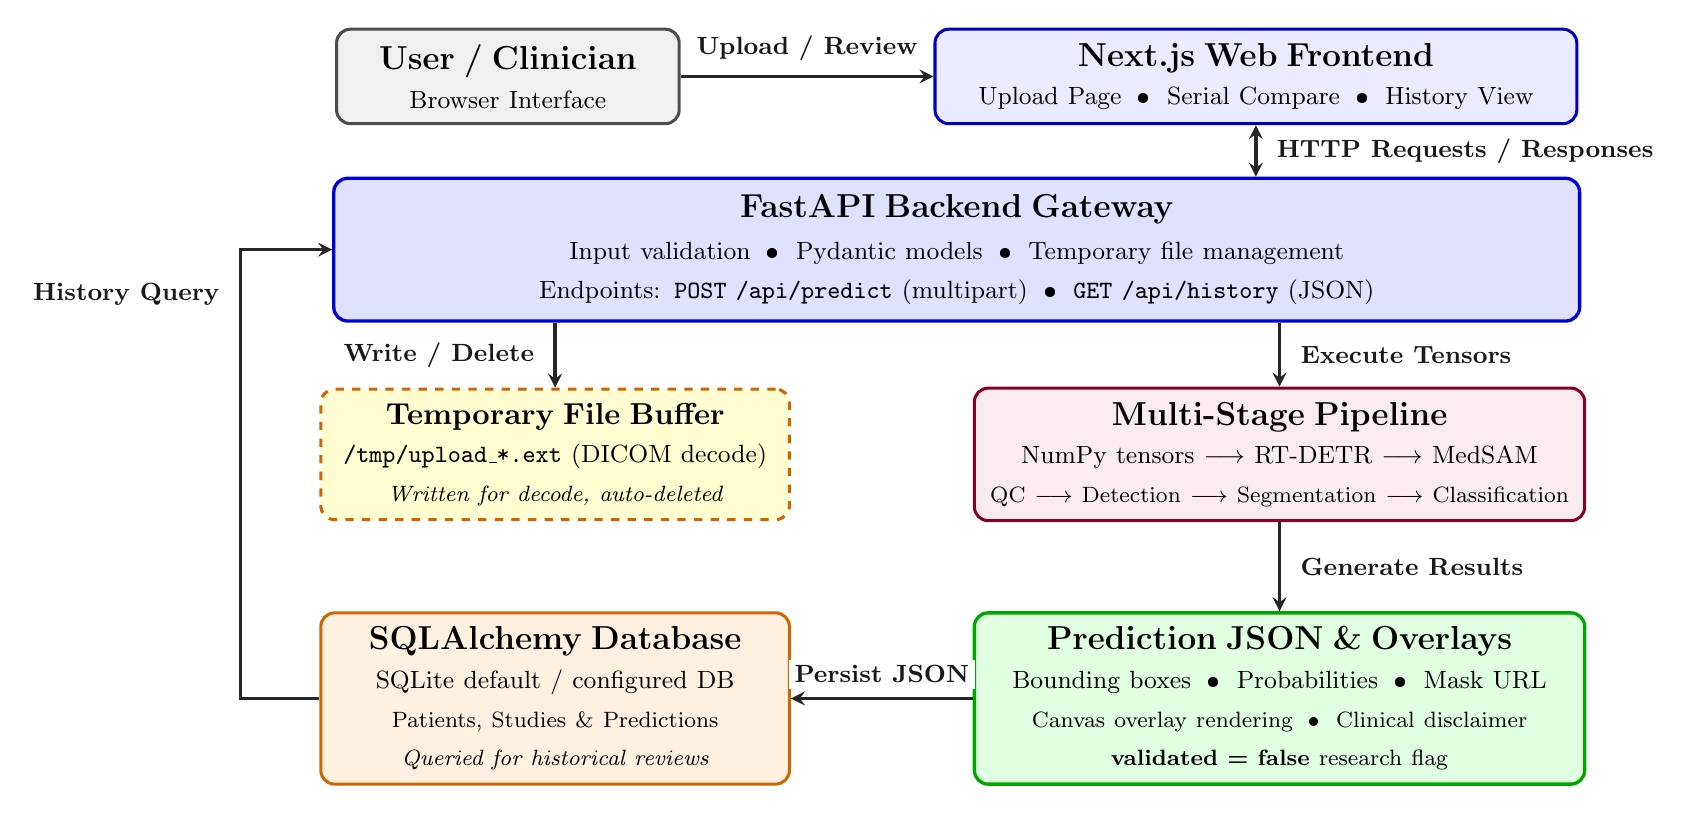
\begin{tikzpicture}[
  actor/.style={draw=black!70, fill=gray!12, rounded corners=5pt, line width=1.1pt, align=center, inner sep=5pt, text width=4.0cm, minimum height=1.2cm},
  front/.style={draw=blue!75!black, fill=blue!8, rounded corners=5pt, line width=1.1pt, align=center, inner sep=5pt, text width=7.8cm, minimum height=1.2cm},
  api/.style={draw=blue!85!black, fill=blue!12, rounded corners=5pt, line width=1.2pt, align=center, inner sep=6pt, text width=15.4cm, minimum height=1.4cm},
  tempbox/.style={draw=orange!80!black, fill=yellow!18, dashed, rounded corners=5pt, line width=1.1pt, align=center, inner sep=5pt, text width=5.6cm, minimum height=1.4cm},
  pipebox/.style={draw=purple!70!black, fill=purple!8, rounded corners=5pt, line width=1.1pt, align=center, inner sep=5pt, text width=7.4cm, minimum height=1.4cm},
  dbbox/.style={draw=orange!80!black, fill=orange!12, rounded corners=5pt, line width=1.1pt, align=center, inner sep=5pt, text width=5.6cm, minimum height=1.6cm},
  jsonbox/.style={draw=green!65!black, fill=green!12, rounded corners=5pt, line width=1.2pt, align=center, inner sep=5pt, text width=7.4cm, minimum height=1.6cm},
  arrow/.style={->, >=stealth, line width=1.2pt, draw=black!85},
  darrow/.style={<->, >=stealth, line width=1.2pt, draw=black!85},
  lbl/.style={font=\fontsize{9pt}{11pt}\selectfont\bfseries, fill=white, inner sep=2pt, text=black!90}
]

  % Row 1: Presentation Layer (y = 0)
  \node[actor] (user) at (-5.7, 0) {
    {\fontsize{11.5pt}{14pt}\selectfont\bfseries User / Clinician}\\[2pt]
    {\fontsize{9pt}{11.5pt}\selectfont Browser Interface}
  };
  \node[front] (ui) at (3.8, 0) {
    {\fontsize{11.5pt}{14pt}\selectfont\bfseries Next.js Web Frontend}\\[2pt]
    {\fontsize{9pt}{11.5pt}\selectfont Upload Page \;\textbullet\; Serial Compare \;\textbullet\; History View}
  };

  % Row 2: API Gateway Layer (y = -2.2)
  \node[api] (api) at (0, -2.2) {
    {\fontsize{12pt}{14.5pt}\selectfont\bfseries FastAPI Backend Gateway}\\[3pt]
    {\fontsize{9pt}{11.5pt}\selectfont Input validation \;\textbullet\; Pydantic models \;\textbullet\; Temporary file management}\\[2pt]
    {\fontsize{9pt}{11.5pt}\selectfont Endpoints: \texttt{POST /api/predict} (multipart) \;\textbullet\; \texttt{GET /api/history} (JSON)}
  };

  % Row 3: Processing & Buffering Layer (y = -4.8)
  \node[tempbox] (temp) at (-5.1, -4.8) {
    {\fontsize{11pt}{13.5pt}\selectfont\bfseries Temporary File Buffer}\\[2pt]
    {\fontsize{9pt}{11.5pt}\selectfont \texttt{/tmp/upload\_*.ext} (DICOM decode)}\\[2pt]
    {\fontsize{8.5pt}{10.5pt}\selectfont\itshape Written for decode, auto-deleted}
  };
  \node[pipebox] (pipe) at (4.1, -4.8) {
    {\fontsize{11.5pt}{14pt}\selectfont\bfseries Multi-Stage Pipeline}\\[2pt]
    {\fontsize{9pt}{11.5pt}\selectfont NumPy tensors $\longrightarrow$ RT-DETR $\longrightarrow$ MedSAM}\\[2pt]
    {\fontsize{8.5pt}{11pt}\selectfont QC $\longrightarrow$ Detection $\longrightarrow$ Segmentation $\longrightarrow$ Classification}
  };

  % Row 4: Persistence & Output Serialization (y = -7.9)
  \node[dbbox] (db) at (-5.1, -7.9) {
    {\fontsize{11.5pt}{14pt}\selectfont\bfseries SQLAlchemy Database}\\[2pt]
    {\fontsize{9pt}{11.5pt}\selectfont SQLite default / configured DB}\\[2pt]
    {\fontsize{8.5pt}{11pt}\selectfont Patients, Studies \& Predictions}\\[2pt]
    {\fontsize{8.5pt}{10.5pt}\selectfont\itshape Queried for historical reviews}
  };
  \node[jsonbox] (json) at (4.1, -7.9) {
    {\fontsize{11.5pt}{14pt}\selectfont\bfseries Prediction JSON \& Overlays}\\[2pt]
    {\fontsize{9pt}{11.5pt}\selectfont Bounding boxes \;\textbullet\; Probabilities \;\textbullet\; Mask URL}\\[2pt]
    {\fontsize{8.5pt}{11pt}\selectfont Canvas overlay rendering \;\textbullet\; Clinical disclaimer}\\[2pt]
    {\fontsize{8.5pt}{10.5pt}\selectfont\bfseries validated = false \textnormal{research flag}}
  };

  % Connectors
  % Row 1
  \draw[arrow] (user) -- node[lbl, above=3pt]{Upload / Review} (ui);

  % Row 1 to Row 2
  \draw[darrow] (ui.south -| 3.8, 0) -- node[lbl, right=5pt]{HTTP Requests / Responses} (api.north -| 3.8, 0);

  % Row 2 to Row 3
  \draw[arrow] (api.south -| temp.north) -- node[lbl, left=5pt]{Write / Delete} (temp.north);
  \draw[arrow] (api.south -| pipe.north) -- node[lbl, right=5pt]{Execute Tensors} (pipe.north);

  % Row 3 to Row 4 (Multi-stage -> Prediction JSON)
  \draw[arrow] (pipe) -- node[lbl, right=5pt]{Generate Results} (json);

  % Row 4 Horizontal: Persist JSON
  \draw[arrow] (json.west) -- node[lbl, above=3pt]{Persist JSON} (db.east);

  % Database to API: History Query
  \draw[arrow] (db.west) -- ++(-1.0, 0) |- node[lbl, pos=0.45, left=5pt]{History Query} (api.west);

\end{tikzpicture}%
}

\newcommand{\FVDatabaseDiagram}{%
\begin{tikzpicture}[node distance=1.2cm and 1.7cm, font=\small]
  \node[fvdata, align=left] (patient) {\textbf{patients}\\id PK\\patient\_id UNIQUE\\dataset\_source\\age, gender\\created\_at};
  \node[fvdata, right=of patient, align=left] (study) {\textbf{imaging\_studies}\\id PK\\patient\_id FK\\image\_id UNIQUE\\study\_number, timehash\\projection, laterality\\fracture\_visible};
  \node[fvdata, right=of study, align=left] (pred) {\textbf{predictions}\\id PK\\image\_id FK\\model\_version\\fracture\_detected\\detections\_json\\classification\_json\\segmentation\_json\\qc\_passed};
  \node[fvdata, below=of study, align=left] (comp) {\textbf{healing\_comparisons}\\patient\_id\\prior/current image ids\\embedding similarity\\pixel diff\\mask Dice / IoU\\registration flag};
  \node[fvdata, below=of pred, align=left] (version) {\textbf{model\_versions}\\name\\version\\checkpoint\\metrics JSON\\active flag};
  \draw[fvarrow] (patient) -- node[above]{1 : N} (study);
  \draw[fvarrow] (study) -- node[above]{1 : N} (pred);
  \draw[fvarrow] (patient) |- (comp);
  \draw[fvline] (study) -- (comp);
  \draw[fvline] (version) -- (pred);
\end{tikzpicture}%
}

\newcommand{\FVValidationDiagram}{%
\begin{tikzpicture}[
  font=\large,
  vbox/.style={draw=blue!75!black, fill=blue!8, rounded corners=6pt, line width=1.3pt, align=center, inner sep=6pt, text width=8.6cm},
  vdec/.style={draw=orange!90!black, fill=yellow!18, rounded corners=6pt, line width=1.3pt, align=center, inner sep=6pt, text width=7.4cm, font=\large\bfseries},
  verr/.style={draw=red!75!black, fill=red!10, rounded corners=5pt, line width=1.2pt, align=center, inner sep=6pt, text width=5.8cm, font=\normalsize},
  vwarn/.style={draw=orange!85!black, fill=orange!12, rounded corners=5pt, line width=1.2pt, align=center, inner sep=6pt, text width=5.8cm, font=\normalsize},
  vresp/.style={draw=green!65!black, fill=green!12, rounded corners=6pt, line width=1.4pt, align=center, inner sep=7pt, text width=8.6cm},
  varrow/.style={->, >=stealth, line width=1.4pt, draw=black!85},
  tagyes/.style={font=\large\bfseries, fill=white, text=green!60!black, inner sep=2pt},
  tagno/.style={font=\large\bfseries, fill=white, text=red!75!black, inner sep=2pt}
]

  % 1. Incoming Request
  \node[vbox] (req) {\textbf{\Large Client Request}\\\normalsize Upload X-ray Image (DICOM, PNG, or JPEG)};
  
  % 2. Gate 1: Pipeline Readiness
  \node[vdec, below=0.55cm of req] (ready) {Is Pipeline Ready?\\\normalsize\normalfont Checkpoint \& service initialized};
  \node[verr, right=1.0cm of ready] (err503) {\textbf{\large HTTP 503 Load Error}\\Model checkpoints or pipeline state missing};
  
  % 3. Gate 2: File Validation
  \node[vdec, below=0.55cm of ready] (valid) {Valid Size \& Format?\\\normalsize\normalfont File size $\le$ 50 MB, valid suffix};
  \node[verr, right=1.0cm of valid] (err413) {\textbf{\large HTTP 413 / 415 Error}\\File oversized or unsupported format};
  
  % 4. Multi-Stage Pipeline Execution
  \node[vbox, below=0.55cm of valid, text width=8.6cm] (exec) {\textbf{\Large Execute Pipeline Stages (try / except)}\\\normalsize Preprocess $\rightarrow$ Detect $\rightarrow$ Segment $\rightarrow$ Classify};
  
  % 5. Fault Isolation: Stage Error Check
  \node[vdec, below=0.55cm of exec] (stage) {Any Stage-Level Error?\\\normalsize\normalfont Exception caught during stage};
  \node[vwarn, right=1.0cm of stage] (errstage) {\textbf{\large Degraded Mode Execution}\\Record stage failure; continue remaining stages};
  
  % 6. Structured Safe Response
  \node[vresp, below=0.55cm of stage] (resp) {\textbf{\Large HTTP 200 Success Response}\\\large\textbf{validated = false} \;\textbullet\; Non-Clinical Disclaimer\\\normalsize Prediction JSON + Mask URL + Heatmaps + Status Flags};

  % Connectors
  \draw[varrow] (req) -- (ready);
  
  \draw[varrow] (ready) -- node[tagno, above]{No} (err503);
  \draw[varrow] (ready) -- node[tagyes, right]{Yes} (valid);
  
  \draw[varrow] (valid) -- node[tagno, above]{No} (err413);
  \draw[varrow] (valid) -- node[tagyes, right]{Yes} (exec);
  
  \draw[varrow] (exec) -- (stage);
  
  \draw[varrow] (stage) -- node[tagno, above]{Yes} (errstage);
  \draw[varrow] (stage) -- node[tagyes, right]{No} (resp);
  
  \draw[varrow] (errstage) |- (resp);

\end{tikzpicture}%
}
